\newpage
\section{Federn}
\label{sec:Federn}

Der Einsatzbereich von Federn ist genau so vielfältig wie die verschiedenen Bautypen, Größen und Werkstoffen. Je nach Funktion können Feder können zug-,druck-, torsion- oder biegebeansprucht werden. 
Die Hauptfunktionen umfassen die Gewährleistung des Kraftflusses und der Kraftverteilung, Speicherung von Energie, Ausdehnungsausgleich, Dampfungssysteme oder Schwingungssysteme. 
Federn werden charakterisiert durch ihre Feder-Kraft-Kennlinie bzw. Moment-Verdrehwinkel-Kennlinie. 

In dieser Arbeit wurde eine rechteckige Blattfeder dimensioniert, gefertigt und als Teil eines Wägesystems kalibriert, siehe Abschnitt \ref{sec:Waegesystem}. Deshalb werden in diesem Abschnitt nur auf biegebeanspruchte, rechteckige Blattfedern näher eingegangen. 

\begin{figure}[htb]
\centering
\subfigure[Rechteckblattfeder (Ansicht und Draufsicht)]
{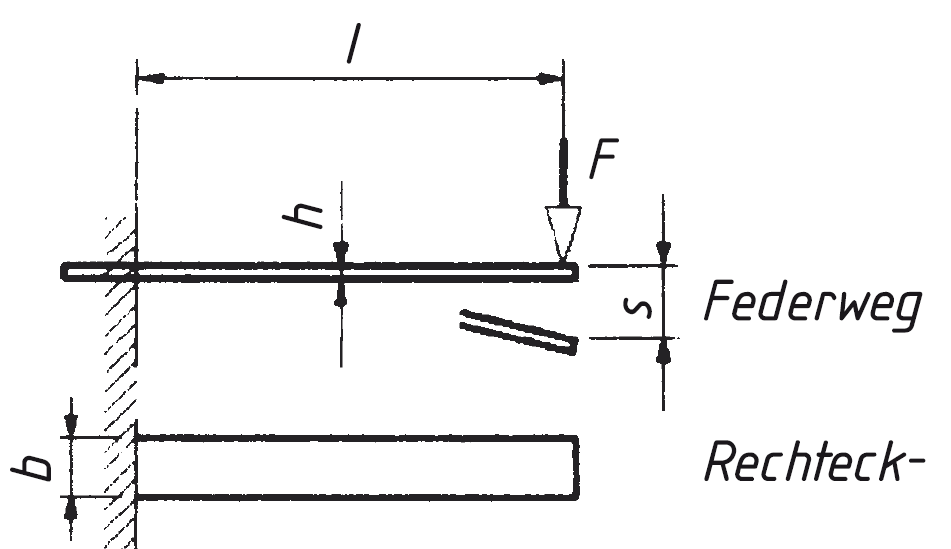
\includegraphics[width=0.4\textwidth]
{Pictures/Federprinzip.png}}
\subfigure[Kraft-Weg-Kennlinien]{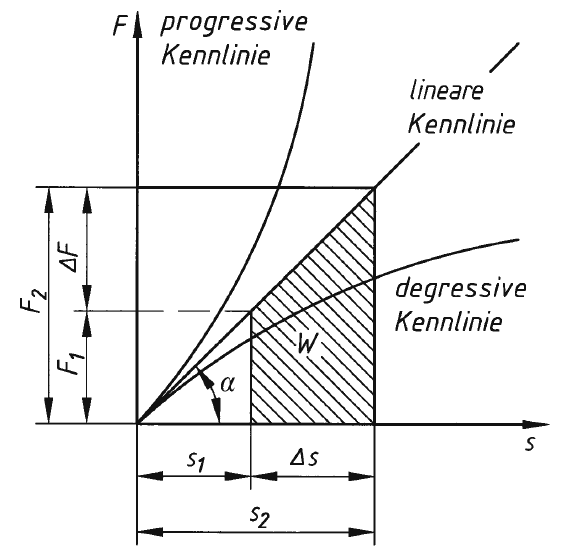
\includegraphics[width=0.4\textwidth]
{Pictures/Kraft-Weg-Kennlinie.png}}
\caption{Blattfeder und Feder-Kennlinien \citep{Wittel2011}}
\label{fig:Federdiagramm}
\end{figure}

Die Abbildung \ref{fig:Federdiagramm}(a) zeigt das Prinzip einer einsetig eingespannten, rechteckigen Blattfeder und \ref{fig:Federdiagramm}(b) drei unterschiedliche Kraft-Weg-Kennlinien. $l$ ist die Länge von der Einspannung bis zum Angriffspunkt der Kraft $F$. $h$ ist die Höhe und $b$ die Breite der Feder. Der Federweg $s$ resultiert aus der Verformung der Feder durch die Belastung mit der der Kraft $F$.

Eine rechteckige Blattfeder verhält sich bei Zunahme der belastenden Kraft $F$ , wie die $lineare~Kennlinie$ im Diagramm aufzeigt. Die Kraft $F$ und der Federweg $s$ sind zu einander proportional. Eine Verdoppelung der Kraft zieht gleichzeitig eine Verdoppelung des Federweges nach sich. Die meisten eingebauten Federn verfügen über eine solche lineare Kennlinie. 

Die aufgenommene Arbeit $W$ ist die Arbeit einer mit $F_1$ vorgespannten Feder, die zusätzlich zu $F_1$ mit $\Delta F$ belastet wird. Die gesamte Kraft beträgt $F_2 = F_1 + \Delta F$. Durch die zusätzliche Kraft verbiegt sich die Feder um $\Delta s$ von $s_1$ auf $s_2$. Die aufgenommene Arbeit $W$ und in Abbildung \ref{fig:Federdiagramm}(b) markierte Fläche errechnet sich zu :

\begin{equation}
W = \frac{1}{2} (F_1 + F_2) \Delta s.
\label{Federarbeit}
\end{equation}


Die Federrate $R$ ist das Verhältnis von der belastender Kraft $F$ zum Federweg $s$:

\begin{equation}
R = tan (\alpha)= \frac{\Delta F}{\Delta s}
\label{eq:Federrate}
\end{equation}


Wie Abbildung \ref{fig:Federrate} zeigt, haben harte Federn eine höhere Federrate. Weiche Feder besitzen hingegen eine kleinere Federrate. 


\begin{figure}[htb]
\centering
\subfigure[Federrate $R$ \citep{Ettemeyer2007}]
{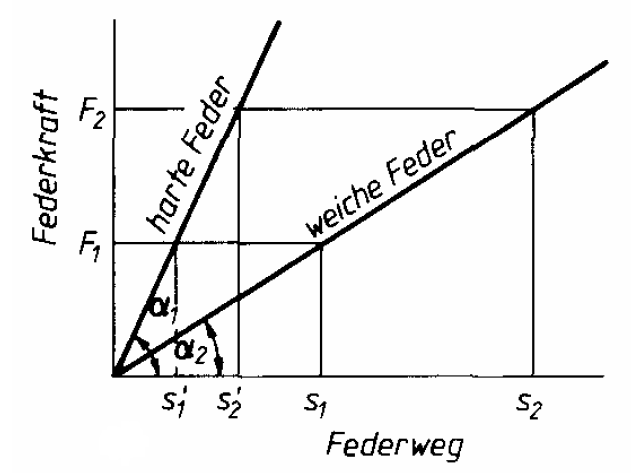
\includegraphics[width=0.52\textwidth]
{Pictures/Federrate.png}}
\subfigure[Federungsarbeit mit Reibungs-Hysterese\citep{Wittel2011}]
{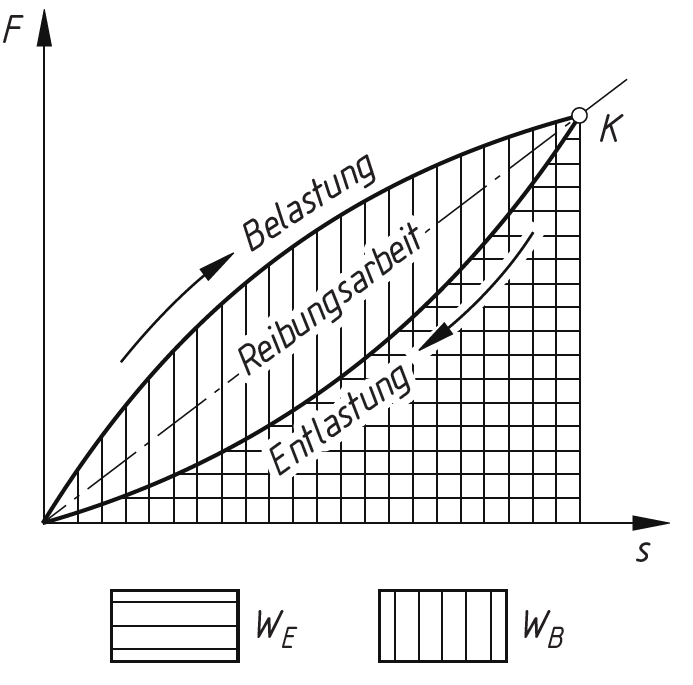
\includegraphics[width=0.4\textwidth]
{Pictures/Federwirkungsgrad.png}}
\caption{Federrate und -wirkungsgrad}
\label{fig:Federrate und -wirkungsgrad}
\end{figure}


Die Biegespannung $\sigma_b$ ist das Verhältnis von der Feder aufzunehmendes Biegemoment $M$ zum Widerstandsmoment $W$. Die Formel für die Biegespannung lautet:

\begin{equation}
\sigma_b = \frac{M}{W}= \frac{6 F l}{b h^2}.
\label{eq:Biegespannung}
\end{equation}

Die maximale Biegespannung ist vom eingesetzten Material und von dem Federtyp abhängig. Die Formel lautet:

\begin{equation}
\sigma_{b,zul} \approx 0,7 \cdot R_m .
\label{eq:Biegespannung}
\end{equation}

Die Sicherheit für die Feder ist definiert als Verhältnis aus der  der maximal zulässigen Biegespannung und maximal auftretenden Biegespannung:

\begin{equation}
S:= \frac{\sigma_{b,zul}}{\sigma_{b,max}};
\label{eq:Biegespannung}
\end{equation}

Für rechteckige Blattfeder ergibt sich für den Federweg $s$ am Ende der Feder zu: 

\begin{equation}
s = 4 \frac{l^3}{b h^3} \frac{F}{E}.
\label{eq:Federweg}
\end{equation}

Hierbei ist $E$ das Elastizitätsmodul des verwendeten Werkstoffes. 

Der Federwirkungsgrad jeder realen Feder ist kleiner als 1. Innere und äußere Reibung führen dazu, dass die zur Belastung aufzuwendende Arbeit $W_B$ größer ist als die Arbeit zur Entlastung $W_E$ der Feder, siehe Abbild \ref{fig:Federrate und -wirkungsgrad}(b). Die Formel für $\eta_F$ lautet:

\begin{equation}
\eta_F = \frac{W_E}{W_B}.
\label{eq:}
\end{equation}

Die Auslegung für die verwendete Feder erfolgt im Abschnitt \ref{sec:Waegesystem}. Für weitere Literatur zum Thema Federn wird auf die Litatur \citep{Wittel2011} und \citep{Ettemeyer2007} verwiesen. 
